\documentclass[11pt,a4paper]{article}

\usepackage{../../../latex/Cours}
\usepackage{listings,tcolorbox}
\usepackage[top=2.2cm, bottom=1cm, left=2cm , right=1.5cm]{geometry}
\begin{document}
\input{\detokenize{../../../latex/Macros.tex}}

%Titre de la fiche d'activité(s) et niveau de la classe
\Activites{\web\; -- C10 : Le Web}{\Pre}
\htmlmode

%Nom de la première activité
\setcounter{numact}{2}
\Act{Une courte introduction à css}{\recherche \; \ordi}

\QListe
\item \textbf{Exemple introductif} \\
Le {\sc css} est un langage permettant de définir les propriétés graphiques (couleurs, bordure, taille, \dots) des éléments d'une page {\sc html}.
\begin{enumerate}
	\item[\textbf{(1)}] \textbf{définir un style} \\
	      Un style se définit en donnant une liste de \textit{propriétés} et leurs \textit{valeurs} séparés par le caractère {\tt :}. Par exemple : \\
	      \texttt{color : blue; font-style : italic;} \\
	      défini un style dans lequel les éléments sont bleus ({\tt color : blue}) et en gras ({\tt font-weight : bold}).
	\item[\textbf{(2)}] \textbf{indiquer les éléments de la page auquel ce style s'applique} \\
	      Une première méthode pour appliquer un style à un élément d'une page consiste à spécifier ce style directement dans l'attribut \texttt{style} de cette élément.
	      Par exemple pour appliquer le style défini ci-dessus à une balise  {\tt <h1>\dots </h1>} :
	      \begin{lstlisting}
<h1 style="color : blue; font-style:italic">Ce titre apparait en bleu et en italique</h1>
\end{lstlisting}
\end{enumerate}
\SQListe
\item Reprendre votre page html. Modifier à votre convenance l'apparence du 
titre de la page (balise {\tt <h1> \dots </h1>}) \\
\aide \; En fin de document vous trouverez une liste non exhaustive de propriétés et de valeurs possibles pour ces propriétés.
\item De même modifier l'apparence des sous titres de votre page (balise {\tt <h2> \dots </h2>}).
\item Encadrer les sous-titres de votre page en ajoutant {\tt border : 1pt solid;} dans le style des balises {\tt <h2> \dots </h2>}.
\item En combien d'endroits a-t-il fallu modifier votre document pour faire cette modification ?
\FinListe

\item \textbf{Définition d'un style dans l'entête de la page}\\
Pour appliquer un style on peut aussi définir le style dans l'entête du document c'est à dire entre les balises \texttt{<head>} et \texttt{</head>}. La définition de la feuille de style doit elle même se trouver entre \texttt{<style>} et \texttt{</style>}. On spécifie alors à quels éléments s'applique le style puis le style lui même (c'est à dire la liste des propriétés avec leurs valeurs). Voici par exemple un des titres de niveau bleu et en italique :
\begin{itemize}
	\item Dans l'entête (donc entre \texttt{<head>} et \texttt{</head>}), on défini le style :
	      \begin{lstlisting}
    <style>
        h2 {color : blue; font-style : italic}
    </style>
\end{lstlisting}
	      \danger \; Remarquer que le style doit être écrit entre accolades ({\tt \{} et {\tt \}}).
	\item Dans le corps du document, le style est automatiquement appliqué aux éléments.
	      \begin{lstlisting}
<body>
<h2> Ce sous-tire sera en bleu et en italique </h2>
...
<h2> Ce sous-titre aussi !<h2>
</body>
\end{lstlisting}
\end{itemize}
Cette méthode présente un avantage par rapport à la technique précédente : il suffit de modifier le style à un seul endroit (dans l'entête) pour modifier tous les éléments de la page auquel il s'applique.
\SQListe
\item Utiliser cette nouvelle méthode pour modifier le style des titres et sous-titres de votre page.
\item Modifier de même le style des paragraphes de votre page web, tester notamment les propriétés {\tt margin} et {\tt padding} afin de comprendre comment elles fonctionnent.
\FinListe
\item \textbf{Définition d'un style dans un fichier séparé}\\
Une troisième technique consiste à définir les styles dans un fichier annexe portant l'extension \texttt{.css} puis à ajouter dans l'entête du document \texttt{html} un lien vers cette feuille de style. Par exemple pour obtenir nos titres en bleu et encadrés en rouge,
\begin{itemize}
	\item créer un fichier \texttt{moncss.css}  comportant la ligne :
	      \begin{lstlisting}
h1 {color : blue; border : 1pt solid red}
\end{lstlisting}
	\item Faire appel à ce fichier dans l'entête de la page html :
	      \begin{lstlisting}
    <link rel='stylesheet' type='text/css'  href='moncss.css'>
\end{lstlisting}
	\item Dans le corps du document :
	      \begin{lstlisting}
<body>
<h1>Ce titre va apparaître en bleu et encadré en rouge</h1>
...
<h1>Ce titre aussi</h1>
</body>
\end{lstlisting}
\end{itemize}
Cette méthode possède un nouvel avantage par rapport à la technique précédente : ce même fichier peut être utilisé pour plusieurs pages différentes du site. On peut donc changer complètement l'aspect de toutes les pages de son site en modifiant un seul fichier !
\vspace{0.1cm}

{Sélection des éléments auxquels le style s'applique}\\
Le \og langage \fg \texttt{css} propose un moyen d'identifier les éléments auxquels le style s'appliquera, il s'agit des \textit{sélecteurs} sans entrer dans les détails notons simplement qu'un sélecteur peut être notamment :
\begin{itemize}
	\item[$\bullet$] un nom de balise, c'est l'exemple que nous avons pris ci-dessus, notre style s'applique aux titres de niveau 1, le sélecteur est \texttt{h1}.
	\item[$\bullet$] un nom de classe préfixé par un point (par exemple \texttt{.important}, \texttt{.encadre}, \dots), dans ce cas le style s'appliquera à toutes les éléments html contenant le nom de cette classe dans leur attribut \texttt{class}.
\end{itemize}
Prenons un exemple pour illuster cette façon d'appliquer un style aux élements d'une page, supposons par exemple que nous voulons faire apparaître certains mots d'un texte barrés et en gris (par exemple pour indiquer que ces mots doivent être corrigés). On définit le style sur le sélecteur \texttt{.barre} de la façon suivante :
\begin{lstlisting}[numbers=none]
.barre {text-decoration : line-through; color : gray}
\end{lstlisting}
Puis dans le corps du document on peut appliquer ce style à tous les éléments ayant le nom du sélecteur dans leur attribut \texttt{class}.
\begin{lstlisting}[numbers=none]
<body>
<p>Ce mot est <span class='barre'>barré</span> de même que  <span class='barre'>celui-ci</span></p>
</body>
\end{lstlisting}
\SQListe
\item Créer votre fichier de style css séparé.
\item Modifier votre page html pour intégré ce fichier comme expliqué ci-dessus.
\FinListe
\pagebreak

\item \textbf{Annexe : quelques propriétés et des valeurs possibles} \\
Pour vous aider, voici une liste non exhaustive des valeurs possibles des propriétés en css ainsi que des valeurs possibles.\\
\renewcommand{\arraystretch}{1.5}
\begin{tabularx}{0.94\textwidth}{|c|c|X|}
	\hline
	\textbf{propriétés}       & \textbf{signification}  & \textbf{valeurs possibles}                                     \\
	\hline
	\texttt{color}            & couleur                 & noms (\texttt{red, green, \dots}) ou  code couleur héxadécimal \\
	\hline
	\texttt{font-family}      & police de caractère     & \texttt{times, courier, arial, \dots}                          \\
	\hline
	\texttt{font-size}        & taille de police        & une valeur numérique et son unité (\texttt{pt, px, em, \dots}) \\
	\hline
	\texttt{font-style}       & italique                & \texttt{normal, italic,  \dots}                                \\
	\hline
	\texttt{font-weight}      & épaisseur               & \texttt{normal, bold, light, \dots}                            \\
	\hline
	\texttt{text-align}       & alignement              & \texttt{ left, right, center, justify}                         \\
	\hline
	\texttt{text-decoration}  & modification texte      & \texttt{none, underline, overline, line-through, \dots}        \\
	\hline
	\texttt{background-color} & couleur de fond         & noms (\texttt{red, green, \dots}) ou  code couleur héxadécimal \\
	\hline
	\texttt{background-image} & image de fond           & url d'une image                                                \\
	\hline
	\texttt{list-style-type}  & puce des listes         & \texttt{disc , square , circle }                               \\
	\hline
	\texttt{list-style-type}  & numérotation des listes & \texttt{decimal, lower-roman, upper-roman, \dots}              \\
	\hline
	\texttt{border}           & bordure                 & taille puis motif (\texttt{solid, dotted, dashed}) et couleur  \\
	\hline
	\texttt{margin}           & marge                   & une valeur numérique et son unité (\texttt{pt, px, em, \dots}) \\
	\hline
	\texttt{padding}          & ajustement              & une valeur numérique et son unité (\texttt{pt, px, em, \dots}) \\
	\hline
\end{tabularx} \\
\begin{itemize}
	\item[$\bullet$] Les notions de \texttt{border, margin} et \texttt{padding} font référence à la façon dont les éléments sont affichés dans le navigateur, c'est à dire dans des \og boîtes \fg permettant de délimiter leur contenu. Le terme \texttt{padding} est l'espacement entre le contenu de la boîte et sa bordure. Et la zone situé au délà de la bordure est la marge. Ces concepts sont illustrés sur le schéma ci-dessous :
	      \begin{center}
		      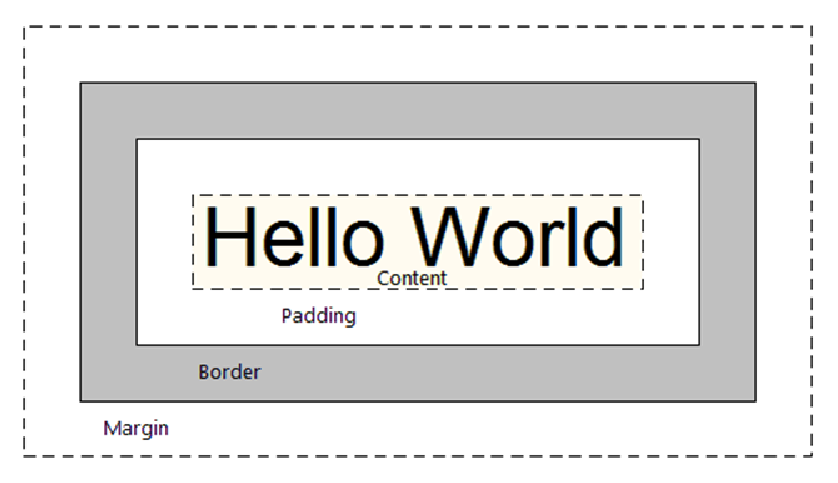
\includegraphics[scale=0.5]{box-model.eps}
	      \end{center}
	\item[$\bullet$] Vous trouverez sur le \textit{Web} des listes complètes des propriétés css, par exemple : \\ {\tt http://www.css-faciles.com/proprietes-css-liste-alphabetique.php}
\end{itemize}
\FinListe
\end{document}